\chapter{Desenvolvimento}

  \section{Base de Dados}

\indent A base de dados KDDcup99 \cite{kdd99} é um dos conjuntos de dados mais utilizados para avaliação de sistemas de detecção de anomalias e detecção de intrusões. A KDD99 foi elaborada à partir dos dados do tráfego gerado artificialmente no DARPA 98, criado pelo Lincoln Laboratory do Instituto Tecnológico de Massachusetts para avaliação de sistemas de detecção de intrusão.

\indent A base contém aproximadamente quatro milhões e novecentos mil vetores de conexões, que são compostos por 42 atributos referentes aos recursos utilizados em cada conexão. Cada vetor de conexão possui uma rotulagem, que pode ser normal ou de algum determinado ataque. Apesar da incerteza no que se refere à efetividade do tráfego gerado artificialmente, este conjunto de dados é utilizado em grande escala na literatura, além disso, a tarefa de clusterização não sofre influência em relação à origem dos dados.

\begin{table}[h]
\centering
\caption{Atributos dos vetores de conexão.}
\vspace{0.5cm}
\begin{tabular}{|r|l|r|l|}
\hline
\textbf{Nº} & \textbf{Nome do Atributo} & \textbf{Nº} & \textbf{Nome do Atributo} \\
\hline                               
1 & Duration 	  & 22 & Count \\
\hline
2 & Protocol\_type & 23 & Srv\_count \\
\hline
3 & Service    	  & 24 & Serror\_rate \\
\hline
4 & Flag          & 25 & Srv\_serror\_rate \\
\hline
5 & Src\_bytes    & 26 & Error\_rate \\
\hline
6 & Dst\_bytes	  & 27 & Srv\_rerror\_rate \\
\hline
7 & Land	  & 28 & Same\_srv\_rate \\
\hline
8 & Wrong\_fragment & 29 & Diff\_srv\_rate \\
\hline
9 & Urgent 	  & 30 & Srv\_diff\_host\_rate \\
\hline
10 & Hot 	  & 31 & Dst\_host\_count \\
\hline
11 & Num\_failed\_logins & 32 & Dst\_host\_srv\_count \\
\hline
12 & Logged\_in   & 33 & Dst\_host\_same\_srv\_count \\
\hline
13 & Num\_compromised & 34 & Dst\_host\_diff\_srv\_rate\\
\hline
14 & Root\_shell  & 35 & Dst\_host\_same\_src\_port\_rate\\
\hline
15 & Su\_attempted & 36 & Dst\_host\_srv\_diff\_host\_rate\\
\hline
16 & Num\_root    & 37	& Dst\_host\_serror\_rate\\
\hline
17 & Num\_files\_creations & 38 & Dst\_host\_srv\_serror\_rate\\
\hline
18 & Num\_shell   & 39 & Dst\_host\_rerror\_rate\\
\hline
19 & Num\_acess\_files & 40 & Dst\_host\_srv\_rerror\_rate\\
\hline
20 & Num\_outbound\_cmds & 41 & Count\\
\hline
21 & Is\_guest\_login & 42 & Attack\_type\\
\hline
\end{tabular}
\end{table}

\begin{table}[h]
\centering
\caption{Ataques agrupados por tipo.}
\vspace{0.5cm}
\begin{tabular}{|l|l|}
\hline
\textbf{Tipos de Ataques} & \textbf{Ataques contidos na KDD99}\\
\hline
DoS &	Back, land, neptune, pod, smurf, teardrop \\
\hline
R2L &	Ftp\_write, guess\_passwd, imap, multihop, phf,\\ & spy, warezclient, warezmaster \\
\hline
U2R &	Buffer\_overflow, load module Pearl, rootkit\\
\hline
Probe &	Ip\_sweep, n\_map, port\_sweep, satan\\
\hline
\end{tabular}
\end{table}

\indent Na Tabela 1 são apresentados os atributos que compõem cada vetor de conexão e o significado de cada atributo. Na Tabela 2 todos tipos de ataques presentes na base de dados são categorizados de acordo com o seu tipo. Esta classificação é importante devido às características semelhantes entre os ataques de mesma categoria, que na clusterização pode refletir em grupos que contenham um ou mais ataques da mesma categoria.

\indent É possível visualizar a forma em que a base de dados é disponibilizada na Tabela 3. Nota-se que há a presença de valores do tipo literal, inteiro e real. Por isso, para aplicar o algoritmo de agrupamento, se faz necessário realizar uma preparação dos dados. A categorização dos dados é exemplificada na Tabela 4, onde os atributos to tipo literal terão seus valores substituídos por valores correspondentes do tipo inteiro. Dessa forma, o algoritmo pode mensurar o valor dos atributos.

\begin{table}[h]
\centering
\caption{Vetor de conexão pré e pós normalização.}
\vspace{0.5cm}
\begin{tabular}{|l|l|}
\hline
\textbf{Estado} & \textbf{Vetor de conexão}\\
\hline
Inicial	 & 0,tcp,http,SF,274,25212,0,0,0,0,0,1,0,0,0,0,0,0,
	\\ & 0,0,0,0,1,6,0.00,0.00,0.00,0.00,1.00,0.00,0.50,39,
	\\ & 137,1.00,0.00,0.03,0.01,0.00,0.00,0.00,0.00.\\
\hline
Normalizado & 0,0,0,0,0,0.00489,0,0,0,0,0,1,0,0,0,0,0,0,0,0,
	   \\& 0,0,0.001957,0.011742,0,0,0,0,1,0,0.5,0.152941,
	   \\& 0.537255,1,0,0.03,0.01,0,0,0,0.\\
\hline

\end{tabular}
\end{table}


\begin{table}[h]
\centering
\caption{Categorização dos protocolos de rede.}
\vspace{0.5cm}
\begin{tabular}{|l|c|}
\hline
\textbf{Protocolo} & \textbf{Valor Categórico}\\
\hline
TCP & 0\\
\hline
UDP & 1\\
\hline
ICMP & 2\\
\hline
\end{tabular}
\end{table}

\indent Após a etapa de categorização, ainda há dados com diferentes ordem de grandezas e unidades de medidas diferentes, tal como, valores reais e valores inteiros muito altos, como, o valor das portas de origem e destino que podem ultrapassar quarenta mil. Em testes empíricos aplicando o K-means na base de dados em que apenas foi realizada a categorização dos dados, a clusterização foi realizada normalmente, porém, os resultados não foram os esperados.

\indent Para realização destes testes, foi elaborada uma base contendo apenas cinquenta vetores de conexão de tráfego normal e cinquenta vetores de um ataque \textit{smurf}. Estes dados foram retirados da própria KDD99 e mantiveram a mesma sequência em que estavam originalmente alocados. Os testes realizados com apenas estes dois grupos, revelaram que os vetores que continham valores muito altos em suas portas de destino, independente de ser do tipo normal ou \textit{smurf}, eram alocados em um grupo muito pequeno que continha em média três objetos. Enquanto o segundo grupo obtinha em média os outros noventa e sete vetores de conexão. Por isso, fez se necessário realizar a normalização para homogenizar os dados em uma mesma escala de valores.

\indent A normalização de dados é um processo que pode ser realizado de diversas maneiras. Neste trabalho foi utilizada a técnica de interpolação linear, onde, assumimos que o domínio de cada atributo está entre os valores máximos e mínimos do atributo presente na base de dados. A normalização linear irá transformar os valores de cada atributo entre [0,1] \cite{goldschmidt2005} \cite{Silva2007}.

\indent Este meio de normalização utiliza os valores máximos e mínimos de cada coluna da base da dados, que serão utilizados para o cálculo do novos valores da base. A seguinte equação representa a normalização por interpolação linear:

\vspace{0.3cm}
\begin{equation}
\label{eq:Interpolação Linear} %Título da equacao
atributo[i][j]' = \frac{atributo[i][j] - min[j]}{\Delta j}
\end{equation}
\vspace{0.3cm}

\noindent onde, assumimos que a base de dados é uma matriz em que $ i $ é o índice da linha, $ j $ o índice da coluna. A variação entre os valores máximos e mínimos é representada por $ \Delta $, onde é composto por $ min $, que representa um vetor contendo o valor mínimo de cada coluna, e por  $ max $, que representa um vetor contendo o valor máximo de cada coluna,

\vspace{0.3cm}
\begin{equation}
\label{eq:Valor de Delta} %Título da equacao
\Delta = max[j] - min[j]
\end{equation}
\vspace{0.3cm}

\noindent o valor normalizado do atributo é representado por $ atributo' $, enquanto o valor inicial é representado por $ atributo $. Na Tabela 3 é apresentado um mesmo vetor de conexão antes e após a normalização.



  \section{Clusterização do Tráfego}

\indent Neste trabalho o algoritmo K-means foi aplicado como uma técnica de divisão e agrupamento do tráfego de rede, para que se possa separar o tráfego normal do tráfego anômalo. Para a realização deste processo, pode-se selecionar somente alguns atributos que exercem maior influência sobre a caracterização do tráfego. Porém, o processo de agrupamento realizado pelo K-means não sofre influência pela quantidade de atributos, deste modo, podemos manter todos os atributos da base, eliminando na fase de treinamento somente o atributo que indica a assinatura do tráfego.

\indent O problema do K-means durante a escolha dos centros iniciais é resolvido com a utilização do K-means++ \cite{arthur2007} que é utilizado de maneira padrão na biblioteca empregada para a execução do algoritmo, e espalha os centros iniciais pela base de dados.

\begin{figure}[!h]
\centering
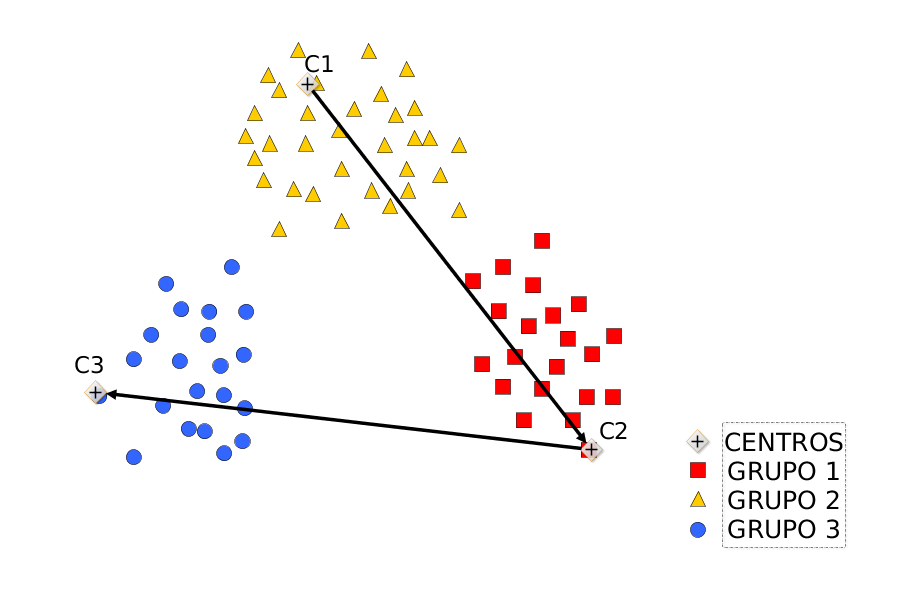
\includegraphics[width = 11cm, height = 8cm]{figuras/kmeans++.png}
\caption{\scriptsize{Distribuição dos centros inicias com Kmeans++.}}
\end{figure}

\indent Primeiramente, o algoritmo escolhe o primeiro centro de forma randômica, depois, é calculada a distância de cada ponto $x$ em relação ao centro já escolhido. E então, é escolhido como o próximo centroide o objeto que possuir a probabilidade proporcional à distância $D(x)^{2}$. Deste modo, os centros inciais são distribuídos nos pontos extremos da base de dados, impossibilitando que iniciem próximos e em um mesmo grupo.

\indent A representação da aplicação do Kmeans++ é demonstrada na Figura 2, no qual, o centro C1 é escolhido randômicamente, C2 é escolhido por ter a maior distância em relação ao C1 e C3 é escolhido por ter a maior distância de C2.

\indent No experimento 1, é apresentado o funcionamento do algoritmo, onde  é realizada a clusterização em uma base de testes contendo três tipos de tráfego: normal e os ataques do tipo \textit{neptune} e \textit{back}, sendo representados respectivamente pelos grupos 1, 2 e 3. Este experimento também é utilizado como fase de treinamento, obtendo-se os seus centros finais para serem utilizados como centro iniciais em outras clusterizações.
  
\begin{figure}[!h]
\centering
\includegraphics[width = 13cm, height = 10cm]{figuras/exp1.png}
\caption{\scriptsize{Experimento 1.}}
\end{figure}

\begin{figure}[!h]
\centering
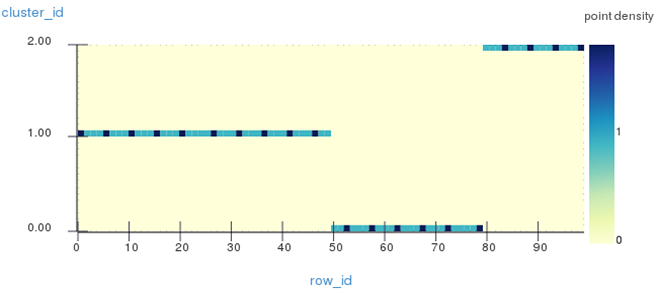
\includegraphics[width = 14cm, height = 8cm]{figuras/densidade2.png}
\caption{\scriptsize{Densidade de elementos do experimento 1.}}
\end{figure}
  
\newpage

\indent No experimento 2 é utilizado o treinamento realizado na clusterização anterior, deste modo, os seus centros finais são aplicados como centros iniciais no experimeto 2, em que os dados estão distribuídos aleatóriamente na base. Diferente do que é realizado no experimento 1, onde os dados foram alocados ordenadamente na base de dados.

\begin{figure}[!h]
\centering
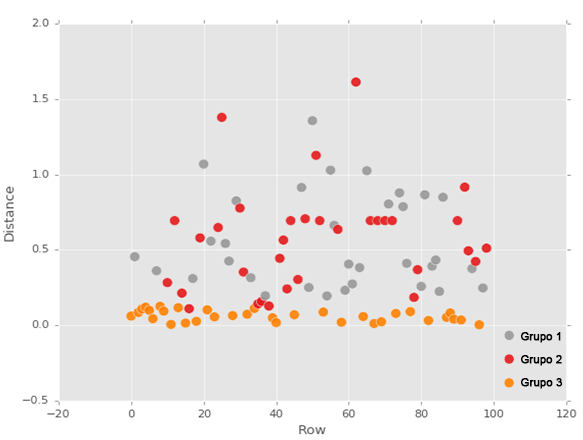
\includegraphics[width = 13cm, height = 10cm]{figuras/aleatorio1.png}
\caption{\scriptsize{Experimento 2.}}
\end{figure}

\begin{figure}[!h]
\centering
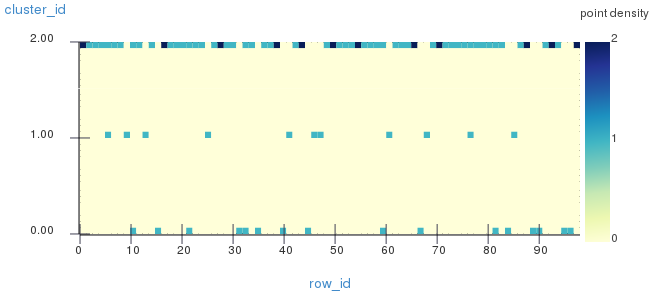
\includegraphics[width = 14cm, height = 8cm]{figuras/densidade1.png}
\caption{\scriptsize{Densidade de elementos do experimento 2.}}
\end{figure}

\indent Nota-se que a clusterização não ocorre como no primeiro experimento, e alguns elementos dos grupos 2 e 3 são alocados ao grupo 1. Nota-se também que há uma grande quantidade de elementos do grupo 1 e 2 que possuem distâncias semelhantes.

\indent Pode-se analisar também a densidade e quantidade de elementos nos três grupos do experimento 1 na Figura 4 e do experimento 2 na Figura 6, sendo possível vizualizar a rescpectiva linha de cada vetor de conexão e suas intercalações na base de dados.

\newpage
    \section{Resultados}
